\section{Parallel Merge Performance}
In order to calculate the efficiency of the parallelised section of the merge algorithm, the cell merge algorithm was timed from the moment the parallel and sequential code diverged to the moment at which they rejoin to output their results. The cell merge for both sequential and parallel merges was tested using the same set of data sources, the size of the data source varied with each iteration having 50, 100, 300, 500, 800, and 1000 sources being used to tessellate and then merge. The merge halting criteria is the error threshold defined by Equation \ref{des:eq:maxerr} in Section \ref{des:sec:merge}. The resulting times for the algorithm to generate the merges can be seen in Figure \ref{res:fig:cvg} with a base 10 logarithmic graph of the results in Figure \ref{res:fig:cvg_1og}
\begin{figure}[H]
\centering
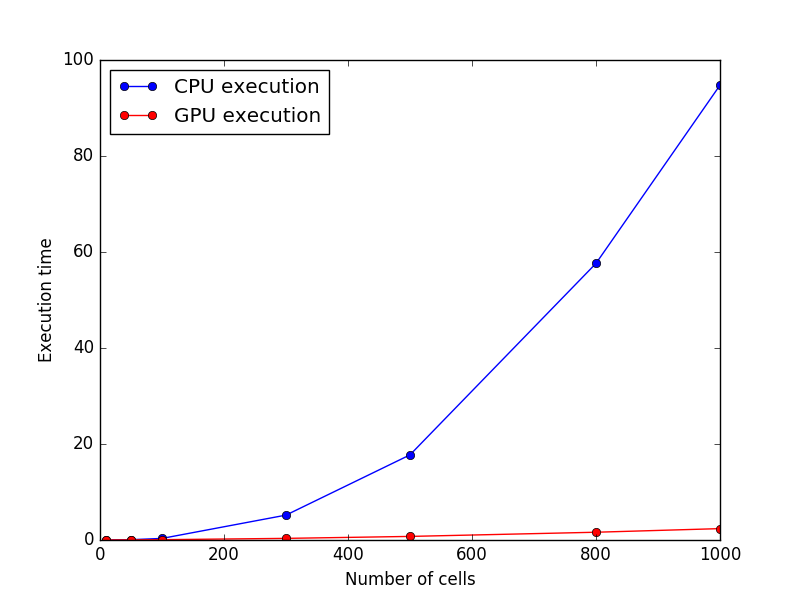
\includegraphics[width=0.8\textwidth]{Images/result_cvg.png}
\caption{A comparison of the computation time of a sequential and parallel execution of the cell merge algorithm.}
\label{res:fig:cvg}
\end{figure}
\begin{figure}[H]
\centering
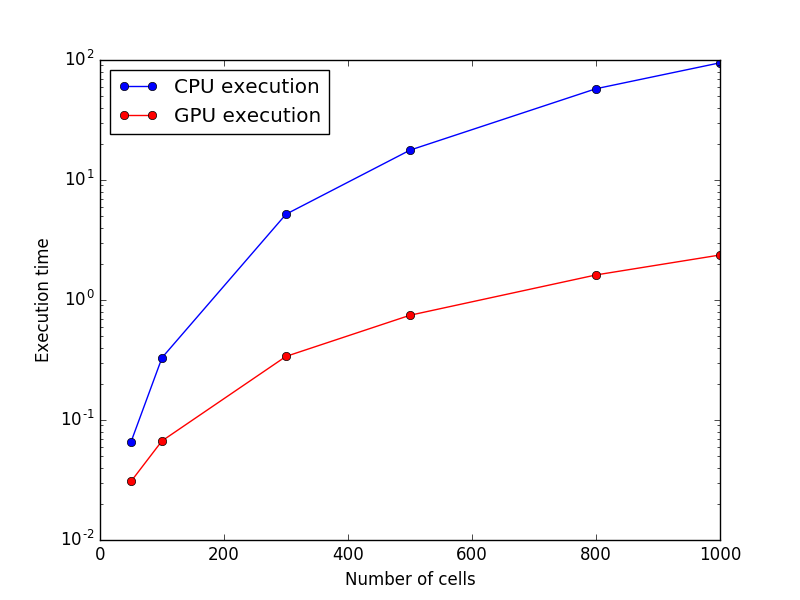
\includegraphics[width=0.8\textwidth]{Images/result_cvg_log.png}
\caption{A logarithmic scale graph of the values depicted in Figure \ref{res:fig:cvg}.}
\label{res:fig:cvg_1og}
\end{figure}
